% Chapter 1

\chapter{Introducción general} % Main chapter title

\label{Chapter1} % For referencing the chapter elsewhere, use \ref{Chapter1}
\label{IntroGeneral}

En este capítulo se contextualiza la enfermedad de Parkinson, la manera habitual de evaluar sus signos motores y se expone la motivación para incorporar análisis automático de video. También se sintetiza el estado del arte en visión por computadora aplicada a trastornos del movimiento y se enuncian los objetivos del trabajo.

%----------------------------------------------------------------------------------------

\newcommand{\keyword}[1]{\textbf{#1}}
\newcommand{\tabhead}[1]{\textbf{#1}}
\newcommand{\code}[1]{\texttt{#1}}
\newcommand{\file}[1]{\texttt{\bfseries#1}}
\newcommand{\option}[1]{\texttt{\itshape#1}}
\newcommand{\grados}{$^{\circ}$}

%----------------------------------------------------------------------------------------

\section{Introducción general al tema}

La enfermedad de Parkinson es un trastorno neurodegenerativo frecuente que compromete principalmente el sistema motor. Entre sus manifestaciones se cuentan la bradicinesia, la rigidez, el temblor en reposo y alteraciones de la marcha y el equilibrio. La gravedad y la evolución de estos signos condicionan la calidad de vida del paciente y las decisiones terapéuticas del profesional de la salud.

En la práctica neurológica se emplean escalas validadas que formalizan la exploración motora. Una referencia ampliamente adoptada es la parte motora de la escala unificada de la Sociedad Internacional de Parkinson y trastornos del movimiento (MDS por su sigla en inglés), conocida en la literatura como MDS-UPDRS parte III, que guía la observación de tareas como movimientos de dedos, postura y marcha \citep{sibley2021video}. Esas puntuaciones son útiles para comparar pacientes y momentos en el tiempo, pero dependen de la pericia del examinador y del contexto de la consulta, factores que introducen variabilidad entre observadores y entre sesiones.

En los últimos años creció el interés por registrar la exploración en video, ya sea en forma presencial o remota, y por apoyar la lectura clínica con algoritmos que midan trayectorias, ritmo y amplitud a partir de las imágenes \citep{sibley2021video,pecoraro2025computer}. Esa línea de trabajo apunta a obtener descriptores cuantitativos reproducibles a partir de grabaciones convencionales, sin reemplazar al médico pero ofreciéndole un respaldo objetivo para el seguimiento.

Para situar visualmente el tipo de tareas que los profesionales solicitan durante la exploración motora, se presentan a continuación ejemplos de 4 ejercicios frecuentemente incluidos en protocolos como la parte motora de la escala MDS-UPDRS. 

En la figura \ref{fig:concepto-finger-tapping} se muestra un ejemplo de finger tapping: toques rítmicos entre el pulgar y el índice. En la imagen se observa la mano en la postura típica de la prueba, que permite al examinador valorar la amplitud, la regularidad y la fatiga del movimiento.

\vspace{0.6em}
\begin{center}
	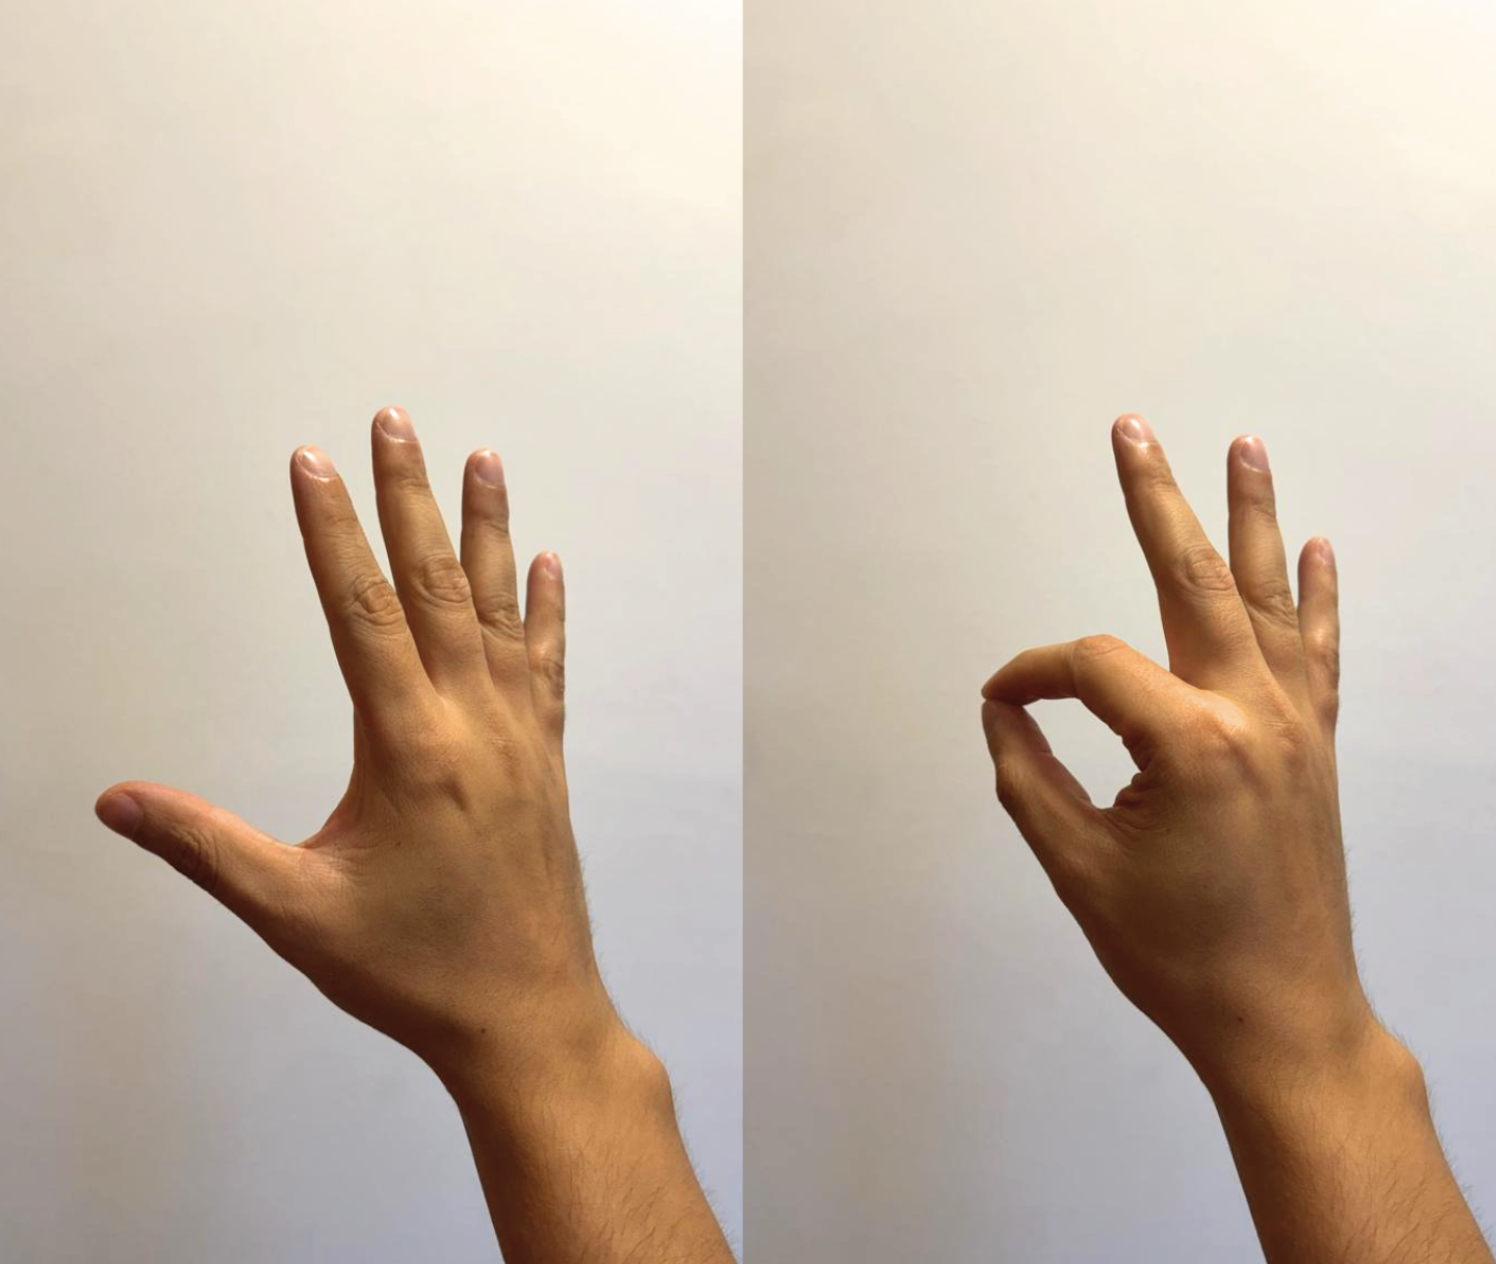
\includegraphics[width=0.88\textwidth]{Figures/cap_1/finger_tapping.png}
	\captionof{figure}{Ejercicio de finger tapping utilizado en la evaluación clínica de movimientos finos de la mano.}
	\label{fig:concepto-finger-tapping}
\end{center}
\vspace{0.4em}

En la figura \ref{fig:concepto-hand-tremor} se ilustra la evaluación del temblor de mano (hand tremor). En ella se observa a una persona de costado con los brazos extendidos hacia el frente, postura utilizada para evaluar los temblores posturales de las extremidades superiores.

\vspace{0.6em}
\begin{center}
	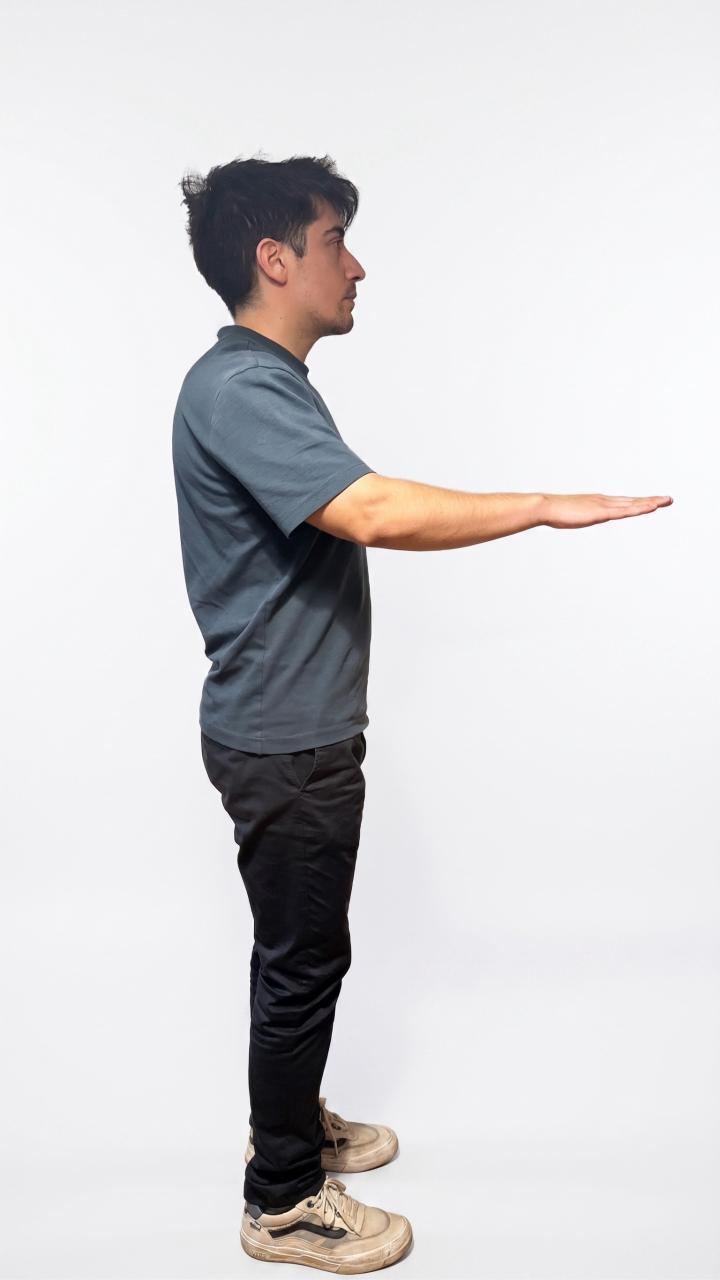
\includegraphics[width=0.34\textwidth]{Figures/cap_1/hand_tremor.jpeg}
	\captionof{figure}{Postura de brazos extendidos hacia el frente para la evaluación del temblor de mano.}
	\label{fig:concepto-hand-tremor}
\end{center}
\vspace{0.4em}

En la figura \ref{fig:concepto-nose-finger} se detalla la prueba nariz-dedo (nose-finger). La secuencia consta de 4 imágenes: inicia con los brazos extendidos, continúa cuando el paciente se toca la nariz con el índice de una mano, vuelve a la postura inicial con ambos brazos extendidos y finaliza cuando se toca la nariz con el índice de la otra mano. Este ejercicio evalúa la precisión del alcance y la coordinación.

\vspace{0.6em}
\begin{center}
	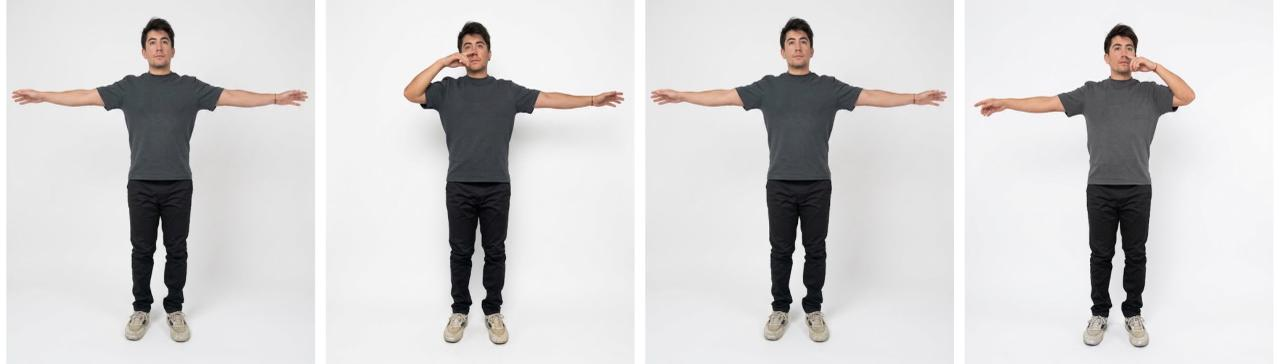
\includegraphics[width=1\textwidth]{Figures/cap_1/nose_finger.jpeg}
	\captionof{figure}{Secuencia de la prueba nariz-dedo, desde la postura de brazos extendidos alternando el contacto con la nariz.}
	\label{fig:concepto-nose-finger}
\end{center}
\vspace{0.4em}

Por último, en la figura \ref{fig:concepto-open-close} se exhibe el ejercicio de apertura y cierre de manos (open-close hands). En la imagen se aprecian las manos de una persona al realizar el ciclo de apertura y cierre. Este ejercicio suele evaluarse en una postura similar a la del temblor de mano, de pie y con los brazos estirados hacia el frente, para analizar la amplitud, la frecuencia y la velocidad de los movimientos.

\vspace{0.6em}
\begin{center}
	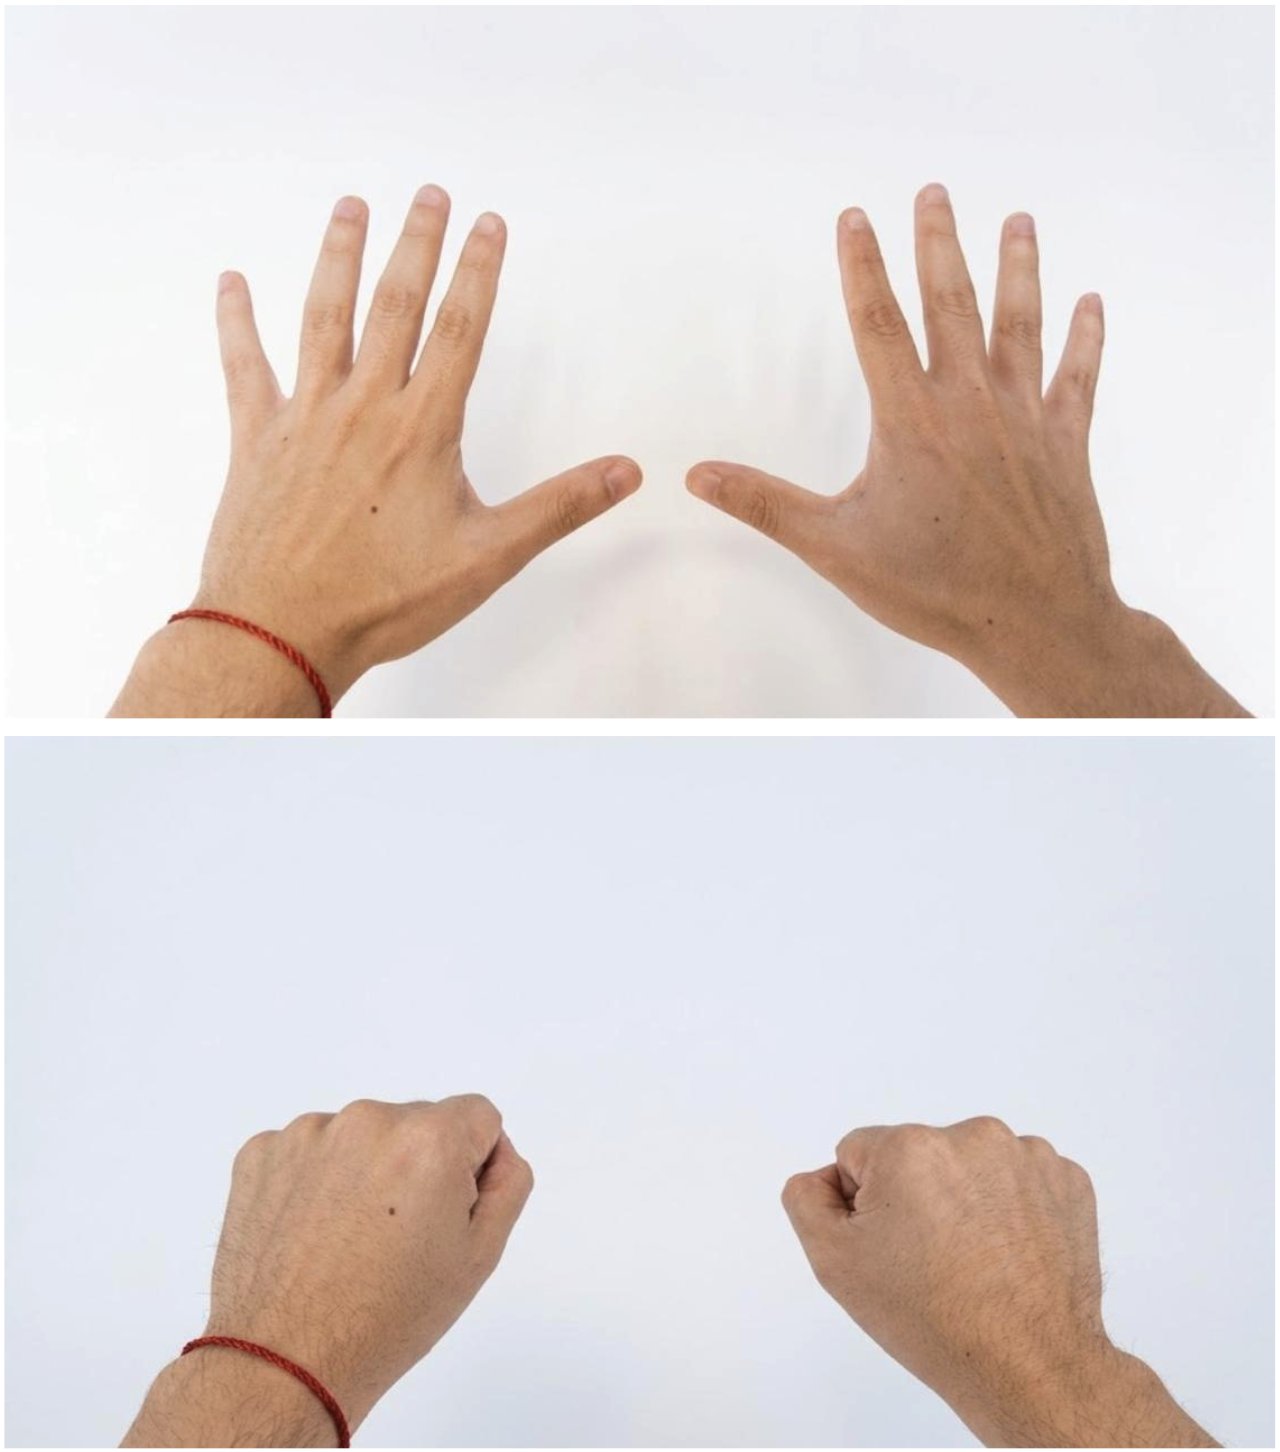
\includegraphics[width=0.54\textwidth]{Figures/cap_1/open_close.png}
	\captionof{figure}{Ejercicio de apertura y cierre de manos, evaluado frecuentemente con los brazos estirados hacia el frente.}
	\label{fig:concepto-open-close}
\end{center}
\vspace{0.4em}

Estas secuencias pueden registrarse en video para analizarlas de forma cuantitativa con herramientas de visión por computadora, como se desarrolla en los capítulos posteriores.

\section{Contexto y motivación}

La motivación del trabajo fue construir una herramienta que, a partir de videos de ejercicios motores, estimara la pose corporal del paciente y derivara métricas asociadas a oscilaciones y regularidad del movimiento. De este modo, se buscó reducir la dependencia exclusiva de la impresión visual humana para apreciar cambios leves o graduales.

La inteligencia artificial y la visión por computadora resultaron adecuadas porque permiten procesar cada fotograma de manera uniforme, conservar el detalle temporal entre cuadros consecutivos y transformar coordenadas articulares en magnitudes interpretables por el personal de salud. Se priorizó un enfoque basado en modelos preentrenados de estimación de pose, alineado con el alcance acordado para el proyecto, que explícitamente no incluyó entrenar redes neuronales desde cero en un conjunto propio de gran escala.

El trabajo culminó con un producto operativo que puede ejecutarse en entorno local y mediante contenedores, y además se desplegó en la nube sobre Google Cloud Platform (GCP) \citep{gcp}, de modo que el acceso al sistema no se limitó a una única máquina de desarrollo. La arquitectura y el procedimiento de despliegue quedaron documentados para facilitar extensiones posteriores, como validación prospectiva frente a lecturas de referencia o adaptaciones institucionales sujetas a marcos éticos y regulatorios propios de cada jurisdicción.

\section{Estado del arte}

La revisión sistemática de Pecoraro, Marsili, Espay, Bologna y di Biase sobre tecnologías de visión por computadora en trastornos del movimiento resume decenas de estudios entre 1984 y 2024 \citep{pecoraro2025computer}. En ese conjunto de investigaciones predominan trabajos sobre la enfermedad de Parkinson y tareas de marcha. Para la estimación de pose sin marcadores físicos aparecen con frecuencia implementaciones basadas en OpenPose \citep{cao2019openpose} y, en menor medida, otras soluciones mediante modelos propios o integraciones desarrolladas para cada estudio.

Los autores destacan que el análisis automático de video alcanzó en muchos informes exactitudes diagnósticas superiores al 80\% frente a etiquetas clínicas, con buena concordancia frente a acelerometría en temblor y distonía, aunque advierten heterogeneidad en condiciones de grabación y en el software empleado, lo que dificulta comparar resultados entre sitios.

En paralelo, el trabajo de Sibley, Girges, Hoque y Foltynie analiza retos metodológicos del análisis de video para cuantificar la severidad motora en Parkinson y el papel de la inteligencia artificial y el aprendizaje automático en ese escenario \citep{sibley2021video}. Concluyen que la evaluación por video es accesible y prometedora, pero que hacen falta muestras amplias y diversas y estándares de desempeño alineados con la práctica clínica antes de generalizar su uso.

Para la estimación de pose en tiempo casi real sobre hardware común, Google publicó el marco MediaPipe, que permite encadenar módulos de visión reutilizables y ajustar el consumo de recursos según el equipo disponible \citep{lugaresi2019mediapipe}. Dentro de ese ecosistema, el modelo de pose corporal ofrece coordenadas normalizadas de puntos anatómicos en dos y tres dimensiones y se utiliza en prototipos de salud y deporte por su equilibrio entre latencia y precisión aceptable para seguimiento de extremidades.

Entre las implementaciones recientes con fines clínicos y de investigación, VisionMD constituyó una plataforma de código abierto destinada al análisis automático de videos de tareas de la parte III de la escala MDS-UPDRS \citep{acevedo2025visionmd}. Mediante aprendizaje profundo localizó al sujeto, permitió marcar con precisión de fotograma el inicio y el fin de cada prueba y derivó variables cinemáticas como amplitud, velocidad y variabilidad a partir del seguimiento markerless de mano y cuerpo con el marco MediaPipe \citep{acevedo2025visionmd,lugaresi2019mediapipe}. El procesamiento se ejecutó en equipos convencionales sin requerir hardware especializado ni envío obligatorio de los videos a servicios en la nube, en contraste con plataformas comerciales cerradas señaladas en la misma publicación.

En estudios piloto con pacientes con enfermedad de Parkinson, los autores reportaron diferencias significativas en métricas de tapping de dedos y otras tareas frente a estados de estimulación cerebral profunda encendida o apagada y frente a niveles de medicación, junto con concordancia inter-evaluador elevada en el uso de la herramienta \citep{acevedo2025visionmd}. Ese trabajo ilustró la viabilidad de cuantificar de forma objetiva pruebas ya incorporadas a la exploración motora estandarizada.

En diciembre del año 2025, como extensión de la plataforma VisionMD, Guarín presentó un método para cuantificar la amplitud y frecuencia del temblor postural de la mano directamente desde videos de teléfonos inteligentes, sin requerir referencias de calibración externas \citep{guarin2025postural}. La propuesta combinó la estimación del diámetro del iris para establecer una escala métrica con modelos de estimación de pose 3D y seguimiento de manos, logrando una fuerte correlación con las puntuaciones clínicas tradicionales y sensibilidad a los efectos del tratamiento.

El prototipo documentado en esta memoria se inscribió en la misma línea de visión sin marcadores físicos basada en MediaPipe Pose y en el análisis de tareas motoras finas a partir de series de puntos clave, pero priorizó un flujo operativo orientado a servicios y despliegue mediante contenedores, como se describe en los capítulos siguientes.

En la tabla \ref{tab:comparativa-enfoques} se contrastan enfoques representativos del estado del arte en cuanto a insumos, salida típica y forma habitual de evaluación reportada en la literatura de revisión. No constituye un inventario exhaustivo de productos comerciales sino una guía conceptual para situar el trabajo desarrollado.

\vspace{0.6em}
\begin{center}
\begin{minipage}{\textwidth}
\centering
\captionof{table}{Enfoques frecuentes para cuantificar el movimiento en Parkinson y contextos afines.}
\label{tab:comparativa-enfoques}
{\setlength{\tabcolsep}{3.5pt}\small
\begin{tabular}{@{}p{0.20\textwidth}p{0.23\textwidth}p{0.26\textwidth}p{0.23\textwidth}@{}}
\toprule
\tabhead{Enfoque} & \tabhead{Datos de entrada} & \tabhead{Salida típica} & \tabhead{Evaluación habitual en la literatura} \\
\midrule
Escalas clínicas (MDS-UPDRS III y otras). & Observación en vivo o video asistido por humano. & Puntuaciones ordinales por ítem. & Consistencia inter-examinador, validez frente a estándares clínicos. \\
Sensores inerciales. & Aceleración o velocidad angular en segmentos corporales. & Series temporales, estimadores de frecuencia y amplitud. & Concordancia con video o con escala clínica. \\
OpenPose u otras redes de pose markerless. & Video monocular o multivista. & Coordenadas 2D o 3D de articulaciones. & Exactitud de clasificación o correlación con medidas de referencia \citep{pecoraro2025computer}. \\
MediaPipe Pose. & Video; modelos preentrenados integrados al marco. & Landmarks normalizados 2D/3D y continuidad temporal en un grafo de procesamiento integrado \citep{lugaresi2019mediapipe}. & Idoneidad para tiempo casi real y bajo consumo en dispositivos habituales, frente a estimadores más pesados \citep{lugaresi2019mediapipe}. \\
\bottomrule
\end{tabular}}
\end{minipage}
\end{center}
\vspace{0.4em}

\section{Objetivos del trabajo}

Con el contexto clínico, la motivación del análisis automático de video y el panorama de la literatura ya expuestos, a continuación se enuncian el objetivo general y los objetivos específicos que guiaron el desarrollo del sistema.

\subsection{Objetivo general}

Diseñar e implementar un sistema de análisis digital de oscilaciones y desempeño motor en videos de ejercicios clínicos asociados a la enfermedad de Parkinson, apoyado en estimación automática de pose y en técnicas de procesamiento de señales e inteligencia artificial, que entregue métricas cuantitativas y visualizaciones comprensibles para apoyar el seguimiento objetivo del movimiento.

\subsection{Objetivos específicos}

\begin{enumerate}
\item Implementar un flujo de ingesta y preprocesamiento de video que alimente de manera estable el estimador de pose y módulos posteriores.
\item Integrar un modelo preentrenado de estimación de pose corporal y un seguimiento temporal de puntos relevantes para los ejercicios considerados.
\item Calcular métricas de amplitud, frecuencia, regularidad y estabilidad postural, u otras derivadas del mismo principio de análisis de series articulares, y agregarlas por sesión para su revisión estadística.
\item Exponer los resultados mediante una interfaz de servicios y una aplicación web que permitan cargar sesiones, inspeccionar gráficos y exportar reportes estructurados.
\item Verificar el comportamiento del software mediante pruebas unitarias y de integración sobre componentes críticos del flujo de procesamiento.
\end{enumerate}

Los criterios de cumplimiento asociados a estos objetivos fueron la ejecución exitosa del flujo completo sobre videos de prueba disponibles para el proyecto, la coherencia de las métricas frente a escenarios controlados o simulados descritos en el capítulo de ensayos, y el paso de la batería de pruebas automatizadas definida en el repositorio del sistema.
